\documentclass[10pt,a4paper]{article}
\usepackage[margin=23mm,top=26mm,bottom=24mm,headheight=14pt,headsep=11pt]{geometry}
\usepackage{fontspec}
\setmainfont{LibertinusSerif-Regular.ttf}[Path=../docs/assets/fonts/,BoldFont=LibertinusSerif-Bold.ttf,ItalicFont=LibertinusSerif-Italic.ttf]
\setsansfont{lmsans10-regular.otf}[BoldFont=lmsans10-bold.otf]
\setmonofont{lmmono10-regular.otf}[Scale=0.82]
\usepackage{unicode-math}
\setmathfont{latinmodern-math.otf}
\usepackage{microtype,booktabs,tabularx,array,ragged2e,amsmath}
\usepackage[table]{xcolor}
\usepackage{graphicx,caption,subcaption,pgfplots}
\pgfplotsset{compat=1.18}
\usepackage[most]{tcolorbox}
\usepackage{fancyhdr,titlesec,fvextra,needspace}
\usepackage[section]{placeins}
\usepackage[numbers,sort&compress]{natbib}
\usepackage{hyperref}
\usepackage[nameinlink,noabbrev]{cleveref}
\definecolor{ink}{HTML}{152631}
\definecolor{accent}{HTML}{087E8B}
\definecolor{slate}{HTML}{8493A5}
\definecolor{muted}{HTML}{65717A}
\definecolor{wash}{HTML}{F2F5F6}
\hypersetup{colorlinks=true,linkcolor=accent,citecolor=accent,urlcolor=accent,
  pdftitle={Business Harness Bench: Evaluating Agents on Business Deliverables},pdfauthor={ERP AI}}
\setlength{\parindent}{0pt}
\setlength{\parskip}{5pt plus 1pt minus 1pt}
\setlength{\emergencystretch}{1.5em}
\linespread{1.06}
\renewcommand{\arraystretch}{1.16}
\newcolumntype{L}{>{\RaggedRight\arraybackslash}X}
\newcolumntype{R}{>{\RaggedLeft\arraybackslash}X}
\captionsetup{font=small,labelfont=bf,labelsep=period,justification=justified,singlelinecheck=false,skip=6pt}
\titleformat{\section}{\large\bfseries\color{ink}}{\thesection.}{0.55em}{}
\titleformat{\subsection}{\normalsize\bfseries\color{ink}}{\thesubsection}{0.55em}{}
\titlespacing*{\section}{0pt}{12pt plus 2pt}{5pt}
\titlespacing*{\subsection}{0pt}{8pt plus 1pt}{3pt}
\pagestyle{fancy}\fancyhf{}
\fancyhead[L]{\small\color{muted}BUSINESS HARNESS BENCH}
\fancyhead[R]{\small\color{muted}Evaluating agents on business deliverables}
\fancyfoot[L]{\footnotesize\color{muted}ERP AI\enspace /\enspace Research}
\fancyfoot[R]{\footnotesize\color{muted}\thepage}
\renewcommand{\headrulewidth}{0.35pt}
\renewcommand{\footrulewidth}{0.35pt}
\fancypagestyle{firstpage}{\fancyhf{}
  \fancyhead[L]{\bfseries ERP AI\quad\normalfont\small\color{muted}RESEARCH}
  \fancyhead[R]{\small\color{muted}Technical report\enspace /\enspace September 2026}
  \fancyfoot[L]{\footnotesize\color{muted}ERP AI\enspace /\enspace Research}
  \fancyfoot[R]{\footnotesize\color{muted}\thepage}
  \renewcommand{\headrulewidth}{1pt}}
\DefineVerbatimEnvironment{verbatim}{Verbatim}{fontsize=\small,breaklines=true,breakanywhere=true,frame=none}
\providecommand{\tightlist}{\setlength{\itemsep}{0pt}\setlength{\parskip}{0pt}}
\newcommand{\ProtoRate}{90.4}
\newcommand{\CodexRate}{84.3}
\newcommand{\ProtoCost}{22.06}
\newcommand{\CodexCost}{219.13}

\begin{document}
\thispagestyle{firstpage}
\begin{center}
{\fontsize{26}{29}\selectfont\bfseries Business Harness Bench\par}
\vspace{5pt}
{\fontsize{17}{21}\selectfont Evaluating Agents on Business Deliverables\par}
\vspace{11pt}
{\bfseries ERP AI}\par
\vspace{3pt}
\href{https://github.com/erphq/business-bench}{\small Code, tasks, scorer, and evaluation evidence}
\end{center}
\vspace{4pt}
\begin{tcolorbox}[colback=wash,colframe=wash,boxrule=0pt,arc=0pt,left=10pt,right=10pt,top=8pt,bottom=8pt]
\small\textbf{Abstract.}\enspaceBusiness agents are useful when the work they deliver is correct, usable, and repeatable. We introduce Business Harness Bench, a runnable benchmark comprising 187 file-based desk tasks across seven categories and 20 application-building tasks with three successive change requests. Desk tasks combine heterogeneous inputs, explicit business rules, reference solutions, and executable checks; build tasks evaluate delivery, permissions, data integrity, and behavior under change. We report a complete desk comparison of Proto with DeepSeek V4.1 Flash and Codex with GPT-5.6-sol, with three attempts per task and a shared frozen scorer. Proto passes 507 of 561 attempts (90.4\%), compared with 473 of 561 (84.3\%) for Codex, a difference of 6.06 percentage points. Captured-usage cost estimates are \$22.06 and \$219.13, respectively. These are results for two configured agent systems on a development task set, not isolated model or harness effects. The release includes task packs, runners, the frozen scorer, and an attempt-level evidence ledger; application tasks are released without a completed build leaderboard.

\end{tcolorbox}
\begin{figure}[!ht]
\centering
\begin{minipage}[t]{0.51\linewidth}
\textbf{A\quad Overall task success}\par\vspace{7pt}
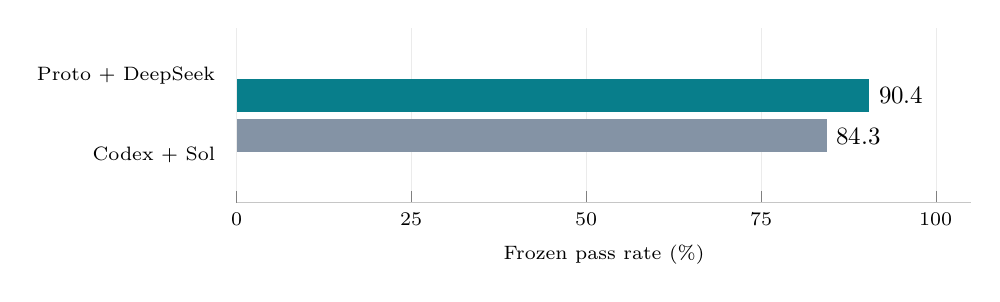
\begin{tikzpicture}
\begin{axis}[width=0.90\linewidth,height=38mm,scale only axis=false,
  xbar,bar width=12pt,xmin=0,xmax=105,ymin=-.6,ymax=1.6,
  axis x line*=bottom,axis y line*=left,y axis line style={draw=none},ytick style={draw=none},xtick={0,25,50,75,100},ytick={0,1},
  yticklabels={Codex + Sol,Proto + DeepSeek},
  tick label style={font=\scriptsize},xlabel={Frozen pass rate (\%)},xlabel style={font=\scriptsize},
  xmajorgrids,grid style={gray!16},axis line style={gray!45},
  nodes near coords,nodes near coords style={font=\small\bfseries,/pgf/number format/fixed,/pgf/number format/precision=1}]
\addplot[fill=accent,draw=none] coordinates {(\ProtoRate,1)};
\addplot[fill=slate,draw=none] coordinates {(\CodexRate,0)};
\end{axis}
\end{tikzpicture}\par
{\scriptsize Captured-usage estimates: \$\ProtoCost{} / \$\CodexCost.}
\end{minipage}\hfill
\begin{minipage}[t]{0.45\linewidth}
\textbf{B\quad Success by repetition}\par\vspace{7pt}
\begin{tikzpicture}
\begin{axis}[width=\linewidth,height=38mm,
  xmin=.8,xmax=3.2,ymin=70,ymax=100,xtick={1,2,3},xticklabels={R1,R2,R3},ytick={70,80,90,100},
  axis x line*=bottom,axis y line*=left,ymajorgrids,grid style={gray!16},axis line style={gray!45},
  tick label style={font=\scriptsize},ylabel={Pass rate (\%)},ylabel style={font=\scriptsize},
  point meta=y,nodes near coords,nodes near coords style={font=\scriptsize,/pgf/number format/fixed,/pgf/number format/precision=1}]
\addplot[accent,thick,mark=*,mark size=2pt] table[x=rep,y=proto]{generated/repetitions.dat};
\addplot[slate,thick,mark=square*,mark size=2pt,nodes near coords style={anchor=north,yshift=-3pt}] table[x=rep,y=codex]{generated/repetitions.dat};
\end{axis}
\end{tikzpicture}\par
{\scriptsize Teal: Proto + DeepSeek. Slate: Codex + Sol.}
\end{minipage}
\caption{\textbf{Complete desk comparison under the shared frozen scorer.} Panel A summarizes all 561 attempts per system; panel B shows the three complete 187-task repetitions. All 1,122 attempts are retained. Costs are API-equivalent estimates, not invoices.}
\label{fig:headline}
\end{figure}

% Generated from paper/benchmark.md and the verified ledger.
\section{Introduction}\label{sec:1}

A business owner delegates a reconciliation because a payment decision depends on it, not because a description of reconciliation is needed. The same distinction applies to an import file, a monthly report, or an internal application: the agent's response is not the deliverable. The relevant question is whether the owner can use what the agent hands back without repairing the work.

Business correctness is often conjunctive. A workbook may show the right total while its formulas fail. An import may be syntactically valid while dropping customers. A payment may match an amount but refer to the wrong invoice. In an application, hiding a button does not enforce authorization. These failures motivate evaluation against explicit delivery contracts rather than fluency, self-reported completion, or activity counts.

Figure \ref{fig:headline} summarizes the complete desk comparison and its repetition-level behavior. The remaining sections define the workload, scoring protocol, category-level findings, and evidence needed to interpret that result.

\section{Benchmark design}\label{sec:2}

Business Bench tests two forms of delegation. In the \textbf{desk track}, an agent receives a folder and a short request, then produces files. In the \textbf{build track}, an agent receives a business requirement and seed data, delivers an application, and applies three changes. Both tracks evaluate the handoff; their scores remain separate because file checks and application acceptance are not interchangeable units.

\subsection{Desk tasks}\label{desk-tasks}

The desk track contains 187 tasks. Inputs include CSV and XLSX exports, text and scanned documents, contextual messages, and occasional databases. Tasks require agents to reconcile inconsistent records, apply supplied policies, preserve required fields, and distinguish supported conclusions from missing evidence. Fixtures are generated business-shaped data, not private customer engagements or a statistically representative sample of business demand.

\begin{table}[!htbp]
\centering\small
\setlength{\tabcolsep}{4pt}
\begin{tabularx}{\linewidth}{@{}>{\hsize=0.75\hsize\linewidth=\hsize\RaggedRight\arraybackslash}X>{\hsize=0.3\hsize\linewidth=\hsize\RaggedRight\arraybackslash}X>{\hsize=1.95\hsize\linewidth=\hsize\RaggedRight\arraybackslash}X@{}}
\toprule
\textbf{Category} & \textbf{Tasks} & \textbf{Representative output} \\
\midrule
Spreadsheet & 41 & Reconciled or calculated workbook \\
Bookkeeping & 36 & Reconciliation, schedule, classification \\
Reports & 30 & Data summary and supported memo \\
Reformatting & 26 & Destination-compatible import file \\
Extraction & 26 & Structured records from documents \\
Drafting & 19 & Business text preserving supplied facts \\
Tooling & 9 & Small file-based tool or static page \\
Total & 187 & Three attempts per reported system \\
\bottomrule
\end{tabularx}
\caption{Composition of the desk track. Each task supplies an ask, workspace, generator, checks, and reference solution. Checks and references remain outside the evaluated agent's container.}
\label{tab:1}
\end{table}


\subsection{Application tasks}\label{application-tasks}

The 20 build tasks cover CRM, inventory, orders, field service, leave, purchase approvals, time tracking, memberships, events, assets, helpdesk, vendors, expenses, quotes, donors, appointments, property maintenance, recruiting, work orders, and point of sale. A shared enterprise baseline addresses delivery, invitations, roles, server-side scope, live dashboards, exact lists and exports, audit metadata, validation, and persistence. Domain-specific checks add the business rules.

Each application receives three successive change requests. The runner carries the prior workspace forward, but invokes a new one-shot turn rather than claiming conversational continuity. Testers recheck existing requirements after each change. Automated probes support delivery checks and produce a tester sheet; they do not establish working permissions or complete acceptance. No completed build leaderboard is reported here.

\subsection{Contribution and scope}\label{contribution-and-scope}

The contribution is an inspectable evaluation package joining portable artifact contracts with application handoff under change. It complements enterprise interaction settings such as WorkArena \citep{workarena}, spreadsheet manipulation in SpreadsheetBench \citep{spreadsheetbench}, and simulated professional work in TheAgentCompany \citep{agentcompany}. EnterpriseClawBench \citep{enterpriseclawbench} evaluates workspace tasks recovered from real workplace sessions. Our inputs are authored fixtures; we do not claim the same source provenance. The benchmark measures configured systems, including models, tools, skills, and execution substrate.

\section{Evaluation protocol}\label{sec:3}

\subsection{Workload and configurations}\label{workload-and-configurations}

The reported comparison covers all 187 desk tasks three times for each system: \textbf{561 attempts per system and 1,122 attempts in total}. Every repetition is retained. The Proto cohort uses runtime revision c8f62dd60 with DeepSeek V4.1 Flash, high reasoning, temperature 0, and DeepSeek-only routing without fallback. Codex uses CLI 0.154.0, GPT-5.6-sol, and high reasoning. Codex sampling is CLI-managed and is not asserted to match Proto's temperature.

The Proto cohort comprises one full repetition and two additional full repetitions of the same runtime. Logical repetition identifiers are preserved in the released ledger. Codex's three full repetitions are reused from its completed benchmark cohort. These are matched task sets under a shared scorer, not simultaneous randomized trials or a same-model harness ablation. Later Proto-versus-Proto development comparisons are outside this release.

\subsection{Frozen artifact scoring}\label{frozen-artifact-scoring}

All attempts are scored with the same \textbf{conservative-v7} package. Each receipt binds the verdict to an original result hash, output-artifact hashes, and the scorer manifest. The release includes the immutable scorer source and task definitions. Export verifies each original result hash and receipt identity; local verification checks every file named by the frozen manifest.

Required checks are conjunctive: a task passes only when every required check passes. Workbook scoring uses native recalculation after cached values are stripped. The frozen scorer includes conservative equivalence checks for alternative valid representations. Original raw verdicts remain separately available; they are not mixed with frozen verdicts in the primary score. There are four original grader-error attempts for Proto and three for Codex, and zero errors under the frozen scorer.

\subsection{Results}\label{results}

\begin{table}[!htbp]
\centering\small
\setlength{\tabcolsep}{4pt}
\begin{tabularx}{\linewidth}{@{}>{\hsize=1.1\hsize\linewidth=\hsize\RaggedRight\arraybackslash}X>{\hsize=0.95\hsize\linewidth=\hsize\RaggedRight\arraybackslash}X>{\hsize=0.95\hsize\linewidth=\hsize\RaggedRight\arraybackslash}X@{}}
\toprule
\textbf{Measure} & \textbf{Proto + DeepSeek V4.1 Flash} & \textbf{Codex + GPT-5.6-sol} \\
\midrule
Repetition 1 & 171/187 & 152/187 \\
Repetition 2 & 167/187 & 160/187 \\
Repetition 3 & 169/187 & 161/187 \\
Frozen score & \textbf{507/561 (90.4\%)} & \textbf{473/561 (84.3\%)} \\
All three attempts pass & 147/187 & 141/187 \\
Original raw score & 447/561 (79.7\%) & 431/561 (76.8\%) \\
\bottomrule
\end{tabularx}
\caption{Complete desk comparison. The primary score is the frozen artifact verdict. Every passing artifact also completed normally; no passing timeout inflates the normal-completion count. Proto has three timeouts overall; Codex has none.}
\label{tab:2}
\end{table}


Proto leads by 34 passing attempts, or \textbf{6.06 percentage points}. The recorded task-clustered bootstrap, which keeps each task's three repetitions together, gives a descriptive 95\% interval of +1.25 to +11.05 points (20,000 resamples; seed 20260916). Related task families and development exposure limit interpretation beyond this workload.

The aggregate exceeds 90\%, but that is not the same as 90\% in every repetition. Proto scores 171, 167, and 169 of 187; its second repetition is 89.3\%. The results support an observed lead on this full desk comparison, not a claim of universal superiority or a passed per-repetition reliability threshold.

\section{Category results and repeatability}\label{sec:4}

\subsection{Where the aggregate lead comes from}\label{where-the-aggregate-lead-comes-from}

\begin{table}[!htbp]
\centering\small
\setlength{\tabcolsep}{4pt}
\begin{tabularx}{\linewidth}{@{}>{\hsize=1.05\hsize\linewidth=\hsize\RaggedRight\arraybackslash}X>{\hsize=0.35\hsize\linewidth=\hsize\RaggedRight\arraybackslash}X>{\hsize=1.45\hsize\linewidth=\hsize\RaggedRight\arraybackslash}X>{\hsize=1.45\hsize\linewidth=\hsize\RaggedRight\arraybackslash}X>{\hsize=0.7\hsize\linewidth=\hsize\RaggedRight\arraybackslash}X@{}}
\toprule
\textbf{Category} & \textbf{Tasks} & \textbf{Proto + DeepSeek} & \textbf{Codex + Sol} & \textbf{Gap (pp)} \\
\midrule
Bookkeeping & 36 & 99/108 (91.7\%) & 98/108 (90.7\%) & +0.9 \\
Drafting & 19 & 49/57 (86.0\%) & 37/57 (64.9\%) & +21.1 \\
Extraction & 26 & 70/78 (89.7\%) & 69/78 (88.5\%) & +1.3 \\
Reformatting & 26 & 74/78 (94.9\%) & 78/78 (100.0\%) & -5.1 \\
Reports & 30 & 81/90 (90.0\%) & 56/90 (62.2\%) & +27.8 \\
Spreadsheet & 41 & 115/123 (93.5\%) & 109/123 (88.6\%) & +4.9 \\
Tooling & 9 & 19/27 (70.4\%) & 26/27 (96.3\%) & -25.9 \\
\bottomrule
\end{tabularx}
\caption{Frozen-scorer results by category. Denominators include all three repetitions. The gap is Proto minus Codex in percentage points; category sizes differ, so category percentages must not be averaged to reconstruct the overall score.}
\label{tab:3}
\end{table}


The largest contribution to the 34-pass aggregate lead comes from \textbf{reports: 81 versus 56 passes}, a gain of 25. Drafting adds 12 passes, spreadsheet work adds six, and bookkeeping and extraction each add one. Codex leads in reformatting by four passes and tooling by seven. The arithmetic is 25 + 12 + 6 + 1 + 1 - 4 - 7 = 34. The overall lead therefore does not imply that Proto wins every category.

Reformatting and tooling are especially useful counterexamples to a universal ranking: Codex passes 78/78 reformatting attempts and 26/27 tooling attempts, compared with Proto's 74/78 and 19/27. These small category samples describe the tested tasks, not independent estimates for every possible import workflow or business tool.

\subsection{Repeatability is a separate measure}\label{repeatability-is-a-separate-measure}

\begin{table}[!htbp]
\centering\small
\setlength{\tabcolsep}{4pt}
\begin{tabularx}{\linewidth}{@{}>{\hsize=1.1\hsize\linewidth=\hsize\RaggedRight\arraybackslash}X>{\hsize=0.95\hsize\linewidth=\hsize\RaggedRight\arraybackslash}X>{\hsize=0.95\hsize\linewidth=\hsize\RaggedRight\arraybackslash}X@{}}
\toprule
\textbf{Passing attempts per task} & \textbf{Proto + DeepSeek} & \textbf{Codex + Sol} \\
\midrule
3 of 3 & 147 & 141 \\
2 of 3 & 29 & 17 \\
1 of 3 & 8 & 16 \\
0 of 3 & 3 & 13 \\
\bottomrule
\end{tabularx}
\caption{Number of tasks with zero, one, two, or three passing attempts. Each column sums to 187 tasks; weighting rows by the number of passes recovers 507 and 473 passing attempts.}
\label{tab:4}
\end{table}


Proto passes all three attempts on \textbf{147/187 tasks (78.6\%)}, versus \textbf{141/187 (75.4\%)} for Codex. It fails all three attempts on three tasks, versus thirteen for Codex. The all-three measure is more demanding than attempt-level accuracy: a task with two successes contributes two passes to the headline rate but is not counted as consistently completed.

At the task-and-repetition pairing level, both systems pass 431 pairs; only Proto passes 76; only Codex passes 42; both fail 12. These counts retain every pair and recover the 34-pass difference. Repetition numbers are bookkeeping identifiers, not matched random seeds or simultaneous trials. Three observations per task do not establish production reliability, and the task-clustered interval in Section \ref{sec:3} should not be read as a guarantee outside this suite.

\section{Worked example: payment reconciliation}\label{sec:5}

\subsection{What the agent receives}\label{what-the-agent-receives}

The \texttt{payments-match-v2} task provides three files: \texttt{bank\_export.csv}, \texttt{open\_invoices.csv}, and \texttt{note.txt}. The owner asks the agent to match the morning's bank credits to open invoices and return three CSV deliverables. The request names the required columns; the note states the business rules. Reference outputs, planted traps, and grader code are not supplied inside the agent container.

\begin{table}[!htbp]
\centering\small
\setlength{\tabcolsep}{4pt}
\begin{tabularx}{\linewidth}{@{}>{\hsize=0.62\hsize\linewidth=\hsize\RaggedRight\arraybackslash}X>{\hsize=1.12\hsize\linewidth=\hsize\RaggedRight\arraybackslash}X>{\hsize=1.26\hsize\linewidth=\hsize\RaggedRight\arraybackslash}X@{}}
\toprule
\textbf{Deliverable} & \textbf{Required fields} & \textbf{Business purpose} \\
\midrule
unpaid.csv & invoice\_id, customer, amount\_outstanding & Show invoices still open and their remaining balances \\
matches.csv & invoice\_id, line\_id, amount\_applied & Record which bank lines settle which invoices \\
unapplied.csv & line\_id, amount, reason & Keep unrelated or closed-invoice credits visible \\
\bottomrule
\end{tabularx}
\caption{The task's three-part delivery contract. A plausible total or explanatory message cannot replace these files or their required row-level relationships.}
\label{tab:5}
\end{table}


\subsection{Rules that change the correct answer}\label{rules-that-change-the-correct-answer}

\textbf{Fees are not always unpaid balances.} Stripe remittances arrive net of 2.9\% plus 30 cents; the note directs the agent to treat the invoice as paid in full. International wires short by up to about 2\% are also treated as paid because intermediary bank charges explain the difference. A generic partial-payment rule would leave an incorrect remainder.

\textbf{A reference is not always authoritative.} One credit names another customer's invoice. The note explicitly gives precedence to the payer and amount. By contrast, a payment identifying an already-closed invoice must remain unapplied; it must not be reassigned merely because another open invoice has a convenient amount.

\textbf{One line can settle several invoices.} A named multi-invoice ACH and a customer-only wire must be distributed across the invoices they actually cover. An exported duplicate must not be applied twice. A genuine 60\% partial payment remains open for its 40\% remainder. Supplier refunds and interest credits belong in the unapplied output, while debits do not.

\subsection{What the checks establish}\label{what-the-checks-establish}

Structural checks enforce output columns and exact sets of open and unapplied identifiers. Numeric comparisons use a one-cent tolerance for outstanding balances. The custom matching check compares both applied totals and contributing bank-line identities; the named duplicate, multi-invoice, fee, wrong-reference, refund, and closed-invoice cases have additional checks.

The contract is not an assertion of perfect row-level accuracy everywhere: the general paid-invoice matching check accepts at least 90\% agreement, while named edge cases impose their own requirements. A task pass means all required checks pass under those declared thresholds. It is not a claim that every conceivable business property has been proved. In the reported full comparison, both systems pass this task in all three repetitions; it illustrates the evaluation contract rather than explaining the aggregate performance gap.

\section{Scoring integrity and application acceptance}\label{sec:6}

\subsection{Original and frozen verdicts}\label{original-and-frozen-verdicts}

The original runner grades outputs immediately after execution. The frozen package is applied separately to retained outputs so both systems use the same scoring definitions. The released ledger preserves both verdicts; passing artifacts are not repaired before the frozen score is recorded.

\begin{table}[!htbp]
\centering\small
\setlength{\tabcolsep}{4pt}
\begin{tabularx}{\linewidth}{@{}>{\hsize=1.1\hsize\linewidth=\hsize\RaggedRight\arraybackslash}X>{\hsize=0.95\hsize\linewidth=\hsize\RaggedRight\arraybackslash}X>{\hsize=0.95\hsize\linewidth=\hsize\RaggedRight\arraybackslash}X@{}}
\toprule
\textbf{Original verdict → Frozen verdict} & \textbf{Proto + DeepSeek} & \textbf{Codex + Sol} \\
\midrule
Pass to pass & 447 & 430 \\
Fail to pass & 56 & 40 \\
Ungraded to pass & 4 & 3 \\
Pass to fail & 0 & 1 \\
Fail to fail & 54 & 87 \\
\bottomrule
\end{tabularx}
\caption{Original-to-frozen verdict transitions across all 561 attempts per system. Original grader errors are labeled ungraded rather than recast as ordinary agent failures. Frozen scoring produced no grader errors.}
\label{tab:6}
\end{table}


Proto's 447 original passes remain passes; 56 original failures and four ungraded attempts pass the frozen scorer, yielding 507. Codex retains 430 of 431 original passes, gains 40 passes from original failures and three from ungraded attempts, yielding 473. The one Codex pass-to-fail transition remains included. These transitions describe evaluator differences on the same artifacts, not improvement from rerunning an agent.

\subsection{The evidence chain}\label{the-evidence-chain}

Each exported attempt carries a hash of its original result, the frozen receipt, the scorer manifest, and retained output artifacts. The exporter checks the original-result hash against the stored file and checks the receipt's scorer identity and verdict. The local verifier checks all files named by the immutable scorer manifest. Hash agreement binds a claim to specific evidence; it does not itself prove that the grader implements the right business rule.

The scorer strips workbook caches before native recalculation, checks readable deliverables, and applies declared structural, numeric, text, and custom checks. It includes conservative equivalences for valid alternative representations. The preserved scorer source makes these decisions inspectable. The original grader and frozen scorer remain separate entry points, so future campaigns must declare which verdict is primary.

\subsection{Build-track acceptance protocol}\label{build-track-acceptance-protocol}

A build sequence has four stages: initial application delivery, then three requested changes to the same workspace. At every stage, the tester verifies the handed-over URL and credentials, evaluates applicable checklist items, and rechecks previously passing requirements. \texttt{RESULT.json} carries the URL, administrator and restricted-user logins, notes, start command, and port. Logins must work; their mere presence in JSON is insufficient.

Acceptance covers record counts and values, invitations, role boundaries, direct-request authorization, live scoped dashboards, validation, audit records, persistence, and domain-specific rules. A hidden UI control is not proof of server-side authorization. A restarted local app can support inspection but does not establish that the originally supplied public URL remained available.

Report initial checklist success, new change-item success, and regressions separately, with time and cost across the sequence. A completed tester sheet must distinguish observed pass, observed failure, and untested requirements. The release provides all 20 task packs and the runner/probe infrastructure, but does not promote automated URL probes into a completed build leaderboard.

\section{Resource use}\label{sec:7}

\begin{table}[!htbp]
\centering\small
\setlength{\tabcolsep}{4pt}
\begin{tabularx}{\linewidth}{@{}>{\hsize=1.1\hsize\linewidth=\hsize\RaggedRight\arraybackslash}X>{\hsize=0.95\hsize\linewidth=\hsize\RaggedRight\arraybackslash}X>{\hsize=0.95\hsize\linewidth=\hsize\RaggedRight\arraybackslash}X@{}}
\toprule
\textbf{Measure} & \textbf{Proto + DeepSeek} & \textbf{Codex + Sol} \\
\midrule
Input tokens & 823,587,929 & 165,959,457 \\
Cached input & 775,672,448 & 150,329,088 \\
Uncached input & 47,915,481 & 15,630,369 \\
Output tokens & 20,910,907 & 4,823,643 \\
Estimated model cost (USD) & 22.06 & 219.13 \\
Median task duration (s) & 124.9 & 135.2 \\
p90 task duration (s) & 455.6 & 403.3 \\
Summed task duration (s) & 113,460.1 & 111,218.8 \\
\bottomrule
\end{tabularx}
\caption{Resources across all 561 attempts per system. Costs are captured-usage API-equivalent estimates under the recorded price table, not subscription invoices or reconciled provider bills. Summed task duration is not elapsed campaign time when attempts run concurrently.}
\label{tab:7}
\end{table}


Proto has lower estimated model cost and median duration, but uses more tokens, slightly more summed task time, and a worse p90. Lower cost therefore does not imply uniformly lower resource use. Cache fractions are token-weighted; uncached totals are reported explicitly.

Proto records 16,954 completed model responses; Codex records 561 task-level usage aggregates, not API requests. These counts are not directly comparable, and separate Codex reasoning-token counts are unavailable. Nine Proto request starts lack completed responses; their additional usage is unknown. First-token latency and turn-start versus intra-turn cache splits are not available.

\section{Validity and limitations}\label{sec:8}

\textbf{Task validity.} Model-assisted authoring and mechanical controls do not replace independent practitioner review or human baselines. The organization developing the suite also develops Proto. Exposure during benchmark-driven development limits claims about unseen generalization.

\textbf{Scoring coverage.} A shared scorer controls grading drift, not all measurement error. Its checks are not exhaustive manual acceptance. Supplemental visual and semantic findings remain separate from the primary score; desk results establish no build-track performance.

\textbf{Configuration and timing.} Models and sampling controls differ, and cohorts were not contemporaneous. Provider behavior, tools, skills, and runtime choices may contribute. This comparison identifies an end-to-end result, not a causal harness-only effect.

\textbf{Reproduction.} Source, tasks, hashes, and score records are released; credentials, traces, historical agent binaries, and raw generated artifacts are not. Hashes identify evidence but cannot reconstruct it. The scorer accepts supplied workspaces, and the runners support new, explicitly configured experiments.

\Needspace{7\baselineskip}

\section{Conclusion}\label{sec:9}

Business Bench evaluates usable business deliverables. On the complete desk comparison, Proto with DeepSeek V4.1 Flash scores \textbf{90.4\%}, versus \textbf{84.3\%} for Codex with GPT-5.6-sol under the same frozen scorer. The release separates correctness, repeatability, execution status, and cost. Application tasks extend the delivery contract to behavior under change; their acceptance results remain unclaimed.

\FloatBarrier
\bibliographystyle{unsrtnat}
\bibliography{references}
\clearpage
\appendix

\section{Running and auditing the benchmark}\label{app:A}

\subsection{Installation and execution}\label{installation-and-execution}

Use Python 3.11 or 3.12 and Docker on a dedicated Linux evaluation host. Install requirements.txt and build the agent and recalculation images with docker/build.sh. Provision a benchmark-owned model login; private agent runtimes are supplied separately. The README contains full commands for each supported adapter and both tracks.

The desk runner mounts only the workspace, isolated home, and read-only adapter into the agent container. References remain on the host. Local-process mode is for development: it does not isolate host-side answers. Network access remains enabled for model requests and permitted tooling; containers are not a guarantee against online discovery of an exposed task set.

Use a fresh result label for each run. The runner refuses to overwrite existing desk labels or attempt directories. Build runs require an explicitly allocated port and a dedicated test environment. Do not expose unreviewed generated applications or mount production credentials. Build tester sheets include generated logins and must remain private.

\subsection{Scoring and verification}\label{scoring-and-verification}

\begin{verbatim}
python -m unittest discover -s tests -v
python bench/export_campaign.py --verify
python bench/release_manifest.py
python scoring/frozen-v7/scorer.py TASK_ID WORKSPACE
\end{verbatim}

Set BENCH\_RECALC\_DOCKER\_IMAGE to the native recalculation image when scoring workbooks. The last command uses the frozen scorer directly; bench/run.py records the original grader's result. Preserve both fields when publishing a new frozen-scored campaign. Never silently substitute a subset of rescored attempts into a raw aggregate.

The canonical manifest digest is:

\begin{verbatim}
b4720db00f2a55461ca70767a4baf8dd2d25aa9d301e8fe22ea13d21ccca358f
\end{verbatim}

The package preserves its original assembly-status text to keep its fingerprint immutable; the subsequent recorded replay covered 1,341 attempts with zero verdict differences. Current export verification checks the receipt and source hashes rather than editing that historical manifest.

\subsection{Release validation}\label{release-validation}

All 187 desk reference-solution/untouched-workspace checks passed with native recalculation; all 20 build-task packs passed structural and seed validation. The strict desk validator reported 28 supplied-fixture byte differences from regenerated outputs despite deterministic repeated regeneration. The supplied inputs remain authoritative and unchanged. Affected tasks are listed in docs/validation.md; byte differences are not assumed semantically harmless.

\section{Reproduction and metric definitions}\label{app:B}

\subsection{Launching a new complete desk run}\label{launching-a-new-complete-desk-run}

The following sequence installs the benchmark and launches the Codex desk matrix after a benchmark-owned login has been provisioned as described in README.md. It makes paid model calls. Use a dedicated Linux host, a unique label, and the exact intended adapter configuration; the example is a new experiment, not a reconstruction of a private historical agent environment.

\begin{verbatim}
python3.12 -m venv .venv
source .venv/bin/activate
pip install -r requirements.txt
bash docker/build.sh
export BENCH_RECALC_DOCKER_IMAGE=bench-recalc:release
python bench/run.py --docker business-bench:release \
  --harness codex-sol --tasks all --runs 3 \
  --parallel 2 --label reproduction-codex
\end{verbatim}

Start with a single-task smoke run under a different label before the full matrix. A different model, provider route, skill inventory, or runtime revision defines a different cell and must be named accordingly. Proto adapters require a separately supplied runtime and isolated model configuration; platform-backed build runs additionally require dedicated test-organization access.

\subsection{Minimum reproducibility record}\label{minimum-reproducibility-record}

\begin{table}[!htbp]
\centering\small
\setlength{\tabcolsep}{4pt}
\begin{tabularx}{\linewidth}{@{}>{\hsize=0.54\hsize\linewidth=\hsize\RaggedRight\arraybackslash}X>{\hsize=1.46\hsize\linewidth=\hsize\RaggedRight\arraybackslash}X@{}}
\toprule
\textbf{Record} & \textbf{Required content} \\
\midrule
Workload & Task identifiers, task/input hashes, repetition mapping \\
Agent environment & Runtime revision, image digest, model route, tools and skills \\
Sampling and budget & Reasoning setting, temperature where controllable, timeout, CPU and memory \\
Scoring & Frozen package digest, original and primary verdicts, grader errors \\
Evidence & Original result hash, output hashes, private artifact retention location \\
Accounting & Captured usage, price assumptions, durations, missing observations \\
\bottomrule
\end{tabularx}
\caption{Minimum record for a new campaign. Missing fields must be disclosed rather than inferred from a successful result. These are prospective requirements, not a claim that every historical environment detail is reconstructible.}
\label{tab:8}
\end{table}


\subsection{Metric definitions}\label{metric-definitions}

\textbf{Attempt pass rate} is the number of frozen passing attempts divided by all attempts in the complete matrix. \textbf{All-three success} is the fraction of task identifiers with three passing attempts. The latter gives one task one vote; the former includes each scheduled attempt.

\textbf{Estimated model cost} sums uncached input, cached input, and output tokens multiplied by their respective per-token prices. Uncached input equals total input minus cached input. The aggregate cache fraction is total cached input divided by total input, not the mean of per-request percentages. Missing usage remains unknown.

\textbf{Duration} is reported at the attempt level. The median describes the center of the observed durations; p90 uses the nearest-rank observation. Summing attempt durations measures aggregate occupied task time and can exceed campaign wall time under concurrency. A positive accuracy gap is stated in percentage points, not as a relative percentage reduction in error.

\subsection{Formal definitions}
For system $h$, let $y_{htr}\in\{0,1\}$ be the frozen pass verdict for task $t$
and repetition $r$. With $T=187$ tasks and $R=3$ repetitions, the reported metrics are
\begin{align}
  \widehat p_h &= \frac{1}{TR}\sum_{t=1}^{T}\sum_{r=1}^{R}y_{htr},
  &\widehat c_h &= \frac{1}{T}\sum_{t=1}^{T}\prod_{r=1}^{R}y_{htr},\label{eq:success}\\
  \Delta_{\mathrm{pp}} &= 100\bigl(\widehat p_{\mathrm{Proto}}-\widehat p_{\mathrm{Codex}}\bigr).
  &&\label{eq:gap}
\end{align}
Here $\widehat p_h$ is attempt-level success and $\widehat c_h$ is all-three success.
The paired bootstrap resamples tasks, retaining all three repetitions within each sampled task;
it does not treat requests or repetitions as independent task families.
For recorded input $I$, cached input $C$, output $O$, and prices per million tokens
$\pi_u$, $\pi_c$, and $\pi_o$, the cost estimate is
\begin{equation}
  \widehat K=\frac{(I-C)\pi_u+C\pi_c+O\pi_o}{10^6}.
  \label{eq:cost}
\end{equation}
Equation~\eqref{eq:cost} accounts only for captured usage. Missing usage is unknown,
not zero, and this quantity is not a subscription invoice.


\end{document}
